\newcommand{\DoNotLoadEpstopdf}{} % no .eps figures; skips a package missing in small TeX installs
\documentclass[10pt,a4paper]{article}

\usepackage[utf8]{inputenc}
\usepackage[T1]{fontenc}
\usepackage{lmodern}
\usepackage[margin=1.7cm,top=1.5cm,bottom=1.6cm]{geometry}
\usepackage{amsmath,amssymb,mathtools}
\usepackage{microtype}
\usepackage{booktabs}
\usepackage{tabularx}
\usepackage{xcolor}
\usepackage[skins]{tcolorbox}
\usepackage{tikz}

\pagestyle{empty}
\setlength{\parindent}{0pt}
\setlength{\parskip}{3pt}
\setlength{\abovedisplayskip}{4pt}
\setlength{\belowdisplayskip}{4pt}
\setlength{\abovedisplayshortskip}{2pt}
\setlength{\belowdisplayshortskip}{2pt}

% Okabe-Ito colours, as in VFI.tex
\definecolor{okblue}{HTML}{0072B2}
\definecolor{okgreen}{HTML}{009E73}
\definecolor{okverm}{HTML}{D55E00}
\definecolor{okorange}{HTML}{E69F00}

\newcommand{\E}{\mathbb{E}}
\newcommand{\ind}{\mathbf{1}}
\newcommand{\code}[1]{\texttt{\detokenize{#1}}}
\newcommand{\hd}[1]{\par\vspace{5pt}{\bfseries\color{okblue!65!black}#1}\par\vspace{1pt}}
\newcommand{\Qbar}{\textcolor{okgreen}{\bar Q}}

\tcbset{sumbox/.style={enhanced,boxrule=0.5pt,arc=1.5pt,left=5pt,right=5pt,top=3pt,bottom=3pt,
        colback=black!2,colframe=black!45,before skip=4pt,after skip=4pt}}

\begin{document}

{\large\bfseries How the RL algorithms make a discrete choice}\par
\vspace{1pt}
{\small Durable-goods model of Fella (2014) in \code{ecomodrl}: the household picks one of 7 durable levels $d'$ and a continuous savings level $a'$ every period.}

% ============================================================== 1
\hd{1\quad The problem}
PPO can draw a category from a list, but DDPG, TD3 and SAC (as implemented in stable-baselines3) can only output a
vector of real numbers in $[-1,1]^n$, a ``Box''. They improve the policy by \emph{gradient ascent on a critic}
$Q(s,u)$, the estimated value of action $u$ in state $s$:
\begin{equation*}
\theta \;\leftarrow\; \theta + \alpha\,\frac{\partial Q(s,u)}{\partial u}\bigg|_{u=\mu_\theta(s)}\frac{\partial \mu_\theta(s)}{\partial \theta},
\end{equation*}
where $\mu_\theta(s)$ is the actor (a neural network). The question is therefore: \emph{how does $Q$ change when
the actor nudges its output a little}, if the choice it controls is discrete?

% ============================================================== 2
\hd{2\quad One action format for everybody: ordinal bins}
Every algorithm outputs $u=(u_0,u_1)\in[-1,1]^2$; the environment turns it into a choice.
\begin{center}
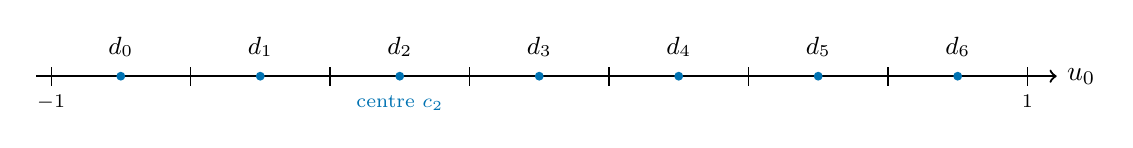
\begin{tikzpicture}[x=6.2cm,y=1cm]
  \draw[thick,->] (-1.03,0) -- (1.06,0) node[right] {$u_0$};
  \foreach \k in {0,...,7} { \draw ({-1+2*\k/7},-0.12) -- ({-1+2*\k/7},0.12); }
  \foreach \k in {0,...,6} {
    \fill[okblue] ({-1+(2*\k+1)/7},0) circle (1.6pt);
    \node[above,font=\small] at ({-1+(2*\k+1)/7},0.12) {$d_\k$};
  }
  \node[below,font=\scriptsize] at (-1,-0.12) {$-1$};
  \node[below,font=\scriptsize] at (1,-0.12) {$1$};
  \node[below,font=\scriptsize,okblue] at ({-1+5/7},-0.12) {centre $c_2$};
\end{tikzpicture}
\end{center}
\vspace{-6pt}
\begin{itemize}\setlength{\itemsep}{1pt}
\item \textbf{Durable:} $[-1,1]$ is cut into 7 equal bins; bin $k=\lfloor (u_0+1)/2\cdot 7\rfloor$ means level $d_k$.
  The levels are \emph{ordered}, so neighbouring bins are neighbouring stocks. If $d_k$ is unaffordable
  (cash-on-hand $z(d_k)\le 0$), the nearest affordable level is used instead (keeping $d$ is always affordable).
\item \textbf{Savings:} $u_1$ sets the consumption share $s\in(0,1]$ of cash-on-hand, so $c=s\,z(d')$ and $a'=z(d')-c\ge 0$.
\end{itemize}
The environment, the evaluation and all figures only ever see this Box. The algorithms differ in how they
\emph{learn} $u_0$.

% ============================================================== 3
\hd{3\quad Why hard bins kill the gradient}
Write $Q_k(s)$ for the value of choosing level $k$ (with the same savings share). Because $u_0$ only matters
through its bin,
\begin{equation*}
Q(s,u_0) = Q_{k(u_0)}(s)\quad\text{is a step function of } u_0, \qquad \frac{\partial Q}{\partial u_0} = 0 \;\text{ almost everywhere.}
\end{equation*}
\begin{center}
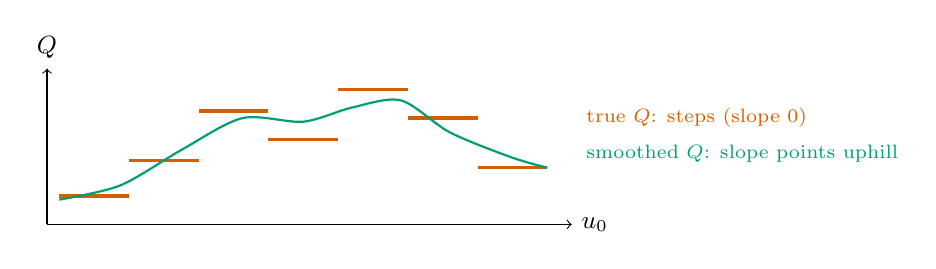
\begin{tikzpicture}[x=3.1cm,y=0.9cm]
  \draw[->] (-1.05,0) -- (1.1,0) node[right,font=\small] {$u_0$};
  \draw[->] (-1.05,0) -- (-1.05,2.2) node[above,font=\small] {$Q$};
  \foreach \k/\q in {0/0.4,1/0.9,2/1.6,3/1.2,4/1.9,5/1.5,6/0.8} {
    \draw[very thick,okverm] ({-1+2*\k/7},\q) -- ({-1+2*(\k+1)/7},\q);
  }
  \draw[thick,okgreen,smooth] plot coordinates {(-1,0.35) (-0.75,0.55) (-0.5,1.05) (-0.25,1.5) (0,1.45) (0.2,1.65) (0.4,1.75) (0.6,1.3) (0.85,0.95) (1,0.8)};
  \node[okverm,font=\scriptsize,anchor=west] at (1.12,1.5) {true $Q$: steps (slope 0)};
  \node[okgreen,font=\scriptsize,anchor=west] at (1.12,1.0) {smoothed $Q$: slope points uphill};
\end{tikzpicture}
\end{center}
\vspace{-4pt}
The fixed adjustment cost makes the steps uneven: staying at the current level is free, every other level costs
$\phi\, d'$. A useful smoothing has to compare whole levels, cost included.

% ============================================================== 4
\hd{4\quad Model-free DDPG, TD3, SAC: the critic smooths for us}
In the model-free variant the critic is itself a neural network $Q_\varphi(s,u)$, fitted by regression to
observed returns. During training the actions are noisy, $u = \mu_\theta(s) + \sigma\varepsilon$ (SAC: drawn from
its Gaussian policy), so the data contain several bins around the actor's output. A neural network cannot reproduce
sharp steps from such data; it fits a smooth curve through them (green line above), whose slope points towards
the better neighbouring level. The algorithm runs \emph{unchanged}.
\textbf{Requirement:} the exploration noise must reach across bin boundaries (bin width $2/7\approx 0.29$). With
almost no noise the critic only sees one bin, its slope is flat, and learning stalls (toy table below). The noise
level $\sigma$ is a tuned hyperparameter, so the tuning step can steer clear of such values.

% ============================================================== 5
\hd{5\quad Post-decision DDPG, TD3, SAC: average over the bins}
The post-decision critic is not a black box: it computes $Q(s,u) = u\big(c,d'\big) + W(a',d',p)$ from the model,
with a network $W$ only for the continuation value. Nothing smooths the step from $u_0$ to $d'$, so the gradient
is \emph{exactly} zero. The fix replaces $Q$ in the actor's objective by its average over the bins under a normal
distribution around the actor's output:
\begin{tcolorbox}[sumbox]
\vspace{-6pt}
\begin{equation*}
\Qbar(s,u) = \sum_{k=0}^{6} P_k(u_0)\, Q\big(s,(c_k,u_1)\big),\qquad
P_k(u_0) = \Phi\!\Big(\frac{e_{k+1}-u_0}{\sigma}\Big) - \Phi\!\Big(\frac{e_k-u_0}{\sigma}\Big),
\end{equation*}
with bin edges $e_k$ (the outer ones are $\mp\infty$), bin centres $c_k$ and the standard normal CDF $\Phi$. Then
\begin{equation*}
\frac{\partial \Qbar}{\partial u_0} = \frac{1}{\sigma}\sum_{k}\Big[\varphi\Big(\frac{e_k-u_0}{\sigma}\Big)-\varphi\Big(\frac{e_{k+1}-u_0}{\sigma}\Big)\Big]\, Q\big(s,(c_k,u_1)\big)\;\neq\;0,
\end{equation*}
\vspace{-12pt}
\end{tcolorbox}
a weighted comparison of the \emph{values of whole levels}, fixed cost included ($\varphi$ is the normal density).
\begin{itemize}\setlength{\itemsep}{1pt}
\item \textbf{TD3, DDPG:} $\sigma = 1/7$ (half a bin): mostly the actor's own bin and its neighbours.
  (TD3's \emph{target} smoothing noise also acts on $u_0$, so its critic targets value a policy that sometimes
  switches level and pays $\phi\,d'$; the tuned noise level keeps this small.)
\item \textbf{SAC:} SAC's policy already is a normal distribution (before a $\tanh$); using its own mean and standard
  deviation, with the edges mapped through $\operatorname{atanh}$, makes $\Qbar$ \emph{exactly} the expected $Q$
  over SAC's own random choice of level, so no extra smoothing is added.
\item Only the actor's objective changes: the critic still learns from the levels that were actually executed.
  Evaluating $Q$ at the 7 bin centres is cheap because $Q$ is a formula plus one small network.
\end{itemize}

% ============================================================== 6
\hd{6\quad PPO: a genuinely discrete policy}
PPO's policy is a probability distribution, and its update uses the log-likelihood trick,
$\nabla_\theta \log \pi_\theta(k,u_1 \mid s)\cdot \hat A$, which needs no derivative of the environment. PPO
therefore gets a \emph{Categorical} distribution over the 7 levels (one logit per level) next to its usual Gaussian
for the savings share. A drawn level $k$ is written into the Box as its bin centre $c_k = -1+(2k+1)/7$, which the
environment maps straight back to $k$; the entropy bonus is the sum of both parts. No smoothing is involved.

% ============================================================== 7
\hd{7\quad Toy experiment (\code{toy_discrete_gradient.py})}
One-step problem with 7 ordered levels: the context is the current level $d$ and a target $x\sim U[0,1]$; the
reward of level $k$ is $-0.05\,(k-6x)^2 - 0.1\cdot\ind\{k\neq d\}$ (plus noise). The ``post-decision'' runs know the
reward of every level exactly. Accuracy = share of contexts where the chosen level is the best one; 4 seeds each.
\begin{center}
\small
\begin{tabular}{@{}lll@{}}
\toprule
Method & Accuracy (4 seeds) & Note \\
\midrule
always stay at $d$ (baseline) & 0.400 & no learning \\
model-free, noise $\sigma=0.02$ & 0.098, 0.806, 0.098, 0.098 & noise too small: 3 of 4 seeds stall \\
model-free, noise $\sigma=0.1$ & 0.726, 0.898, 0.825, 0.812 & critic smoothing works \\
model-free, noise $\sigma=0.3$ & 0.843, 0.830, 0.843, 0.866 & critic smoothing works \\
post-decision, hard bins & 0.164, 0.164, 0.164, 0.164 & gradient exactly 0: the actor never moves \\
post-decision, linear interpolation & 0.871, 0.861, 0.833, 0.881 & compares neighbouring levels only \\
post-decision, average over bins ($\sigma=1/7$) & 0.828, 0.844, 0.859, 0.858 & used in the code (Section 5) \\
\bottomrule
\end{tabular}
\end{center}
Both smoothing rules for the post-decision variant work about equally well here (the width $\sigma$ trades off how
far the actor looks against how much the average blurs the levels); the average over bins is used because it covers
SAC exactly with SAC's own distribution. Hard bins never learn.

% ============================================================== 8
\hd{8\quad Where this lives in the code}
{\small
\begin{tabularx}{\linewidth}{@{}l>{\raggedright\arraybackslash}X@{}}
\toprule
\code{models/durablegoods.py} & \code{controls_from_action}: bins, nearest affordable level, savings share; \code{discrete_action_bins = {0: 7}} \\
\code{algorithms/discrete_actions.py} & \code{gaussian_bin_probs}, \code{expected_bin_q} (Section 5); \code{HybridActorCriticPolicy} (Section 6) \\
\code{algorithms/post_decision/algorithms.py} & actor losses of PD-TD3/DDPG (\code{_pd_td3_train}) and PD-SAC use $\Qbar$ \\
\code{algorithms/training.py} & \code{build_model}: PPO gets the hybrid policy when the model declares bins \\
\bottomrule
\end{tabularx}}

\end{document}
